% JUMP TO LINE 60, 75
\documentclass[preview, margin=0.6in]{standalone}
\usepackage[letterpaper,portrait,top=0.4in, left=0.6in, right=0.6in, bottom=1in]{geometry}

\usepackage{amsmath, amsfonts, amsthm, amssymb}
\usepackage{graphicx, float}
\usepackage{mathtools}
\usepackage{titlesec}
\usepackage{interval}
\usepackage{hyperref}
\usepackage{siunitx}
\usepackage{titling}
\usepackage{vwcol}
\usepackage{setspace}
\usepackage{empheq}
\usepackage{cancel}
\usepackage{esdiff}
\usepackage{multicol}
\usepackage{mdframed}
\usepackage{esdiff}
\usepackage{tikzsymbols}
\usepackage{multicol}
\usepackage{tikz}
\usepackage{varwidth}
\usepackage{parskip}
\usepackage{pgfplots}
\usepackage{pdfpages}

\pgfplotsset{compat=1.18}
\intervalconfig {
	soft open fences
}

\newcommand{\alignedintertext}[1]{%
  \noalign{%
    \vtop{\hsize=\linewidth#1\par
    \expandafter}%
    \expandafter\prevdepth\the\prevdepth
  }%
}

\newtheorem{lemma}{Lemma}

\renewcommand{\qedsymbol}{\Smiley[1.3]}
\newcommand*{\problem}[1]{\section*{Problem #1}}
\newcommand*{\aps}{\section*{AP Corner}}
\newcommand*{\deriv}[1][x]{\ensuremath{\dfrac{\mathrm{d}}{\mathrm{d}#1}}}
\newcommand*{\floor}[1]{\ensuremath{\lfloor #1\rfloor}}
\newcommand*{\lheqzero}{\ensuremath{\underset{\text{L'H}}{\overset{\left[\frac00\right]}{=}}}}
\newcommand*{\lheqinfty}{\ensuremath{\underset{\text{L'H}}{\overset{\left[\frac{\infty}{\infty}\right]}{=}}}}

\DeclareMathOperator{\DNE}{DNE}
\DeclareMathOperator{\sgn}{sgn}

\DeclareMathOperator{\arccsc}{arccsc}
\DeclareMathOperator{\arcsec}{arcsec}
\DeclareMathOperator{\arccot}{arccot}

%opening

\title{\vspace*{-40pt}Problem Set \#53}
\author{Jayden Li}
\date{\today}
% \allowdisplaybreaks
\postdisplaypenalty=100000

\begin{document}
\setstretch{1.25}
\fontsize{12pt}{12pt}\selectfont
\setlength{\abovedisplayskip}{\abovedisplayskip/2}
\setlength{\belowdisplayskip}{\belowdisplayskip/2}
\setlength{\parindent}{0pt}
\setlength{\parskip}{2ex plus 0.5ex minus 0.2ex}
\maketitle

\problem{3}
\begin{itemize}
	\item[(b)]
		$\begin{aligned}[t]
			\sum_{n=0}^{\infty}\frac{(-1)^n \pi ^{2n+1}}{4^{2n+1}(2n+1)!}
			&=\sum_{n=0}^{\infty}\frac{(-1)^n}{(2n+1)!}\left(\frac{\pi}{4}\right)^{2n+1}
			=\sin\left(\frac{\pi}{4}\right)
			=\boxed{\frac{\sqrt{2}}{2}}
		\end{aligned}$
\end{itemize}

\problem{4}
\begin{itemize}
	\item[(a)]
		\begin{equation*}
			\int e^{-x^2}\,\mathrm{d}x
			=\int \sum_{n=0}^{\infty}\frac{\left(-x^2\right)^n}{n!}\,\mathrm{d}x
			=\int \sum_{n=0}^{\infty}\frac{(-1)^n x^{2n}}{n!}\,\mathrm{d}x
			=\boxed{\sum_{n=0}^{\infty}\frac{(-1)^n x^{2n+1}}{(2n+1)n!}+C}
		\end{equation*}

	\item[(b)]
		Let $\displaystyle 
			S
			=\int_{0}^{1}e^{-x^2}\,\mathrm{d}x
			=\left.\sum_{n=0}^{\infty}\frac{(-1)^n x^{2n+1}}{(2n+1)n!}\right|_{0}^{1}
			=\sum_{n=0}^{\infty}\frac{(-1)^n}{(2n+1)n!}
		$.

		Let $S_k$ be the $k$th partial sum of $S$. Then $\displaystyle 
			S_k
			=\sum_{n=0}^{k}\frac{(-1)^n}{(2n+1)n!}
		$.

		Let $a_n$ be the $n$th term of the sum, then let $b_n=\left|a_n\right|=\displaystyle \frac{1}{(2n+1)n!}$.

		By the alternating series estimation theorem, we have:
		\begin{equation*}
			\mathrm{Error}=\left|S-S_k\right|
			\leq \underbrace{b_{k+1}
			=\frac{1}{(2k+3)(k+1)!}\leq 0.001}
		\end{equation*}
		The braced equation always implies the error is less than $0.001$. By calculator, that equation is true when $k\geq4$. Therefore, $S\approx S_4$ within the acceptable error.
		\begin{equation*}
			S_4
			=\sum_{n=0}^{4}\frac{(-1)^n}{(2n+1)n!}
			=1-\frac13+\frac{1}{10}-\frac{1}{42}+\frac{1}{216}
			\approx \boxed{0.747}
		\end{equation*}
\end{itemize}

\problem{5}
\begin{equation*}
    \lim_{x\to0}\frac{e^x-1-x}{x^2}
	=\lim_{n\to\infty}\frac{1+x+\sum_{n=2}^{\infty}\frac{x^n}{n!}-1-x}{x^2}
	=\lim_{x\to0}\sum_{n=2}^{\infty}\frac{x^n}{n!x^2}
	=\lim_{x\to0}\left[\frac{1}{2!}+\sum_{n=3}^{\infty}\frac{x^{n-2}}{n!}\right]
	=\boxed{\frac12}
\end{equation*}

\problem{6}
\begin{center}
	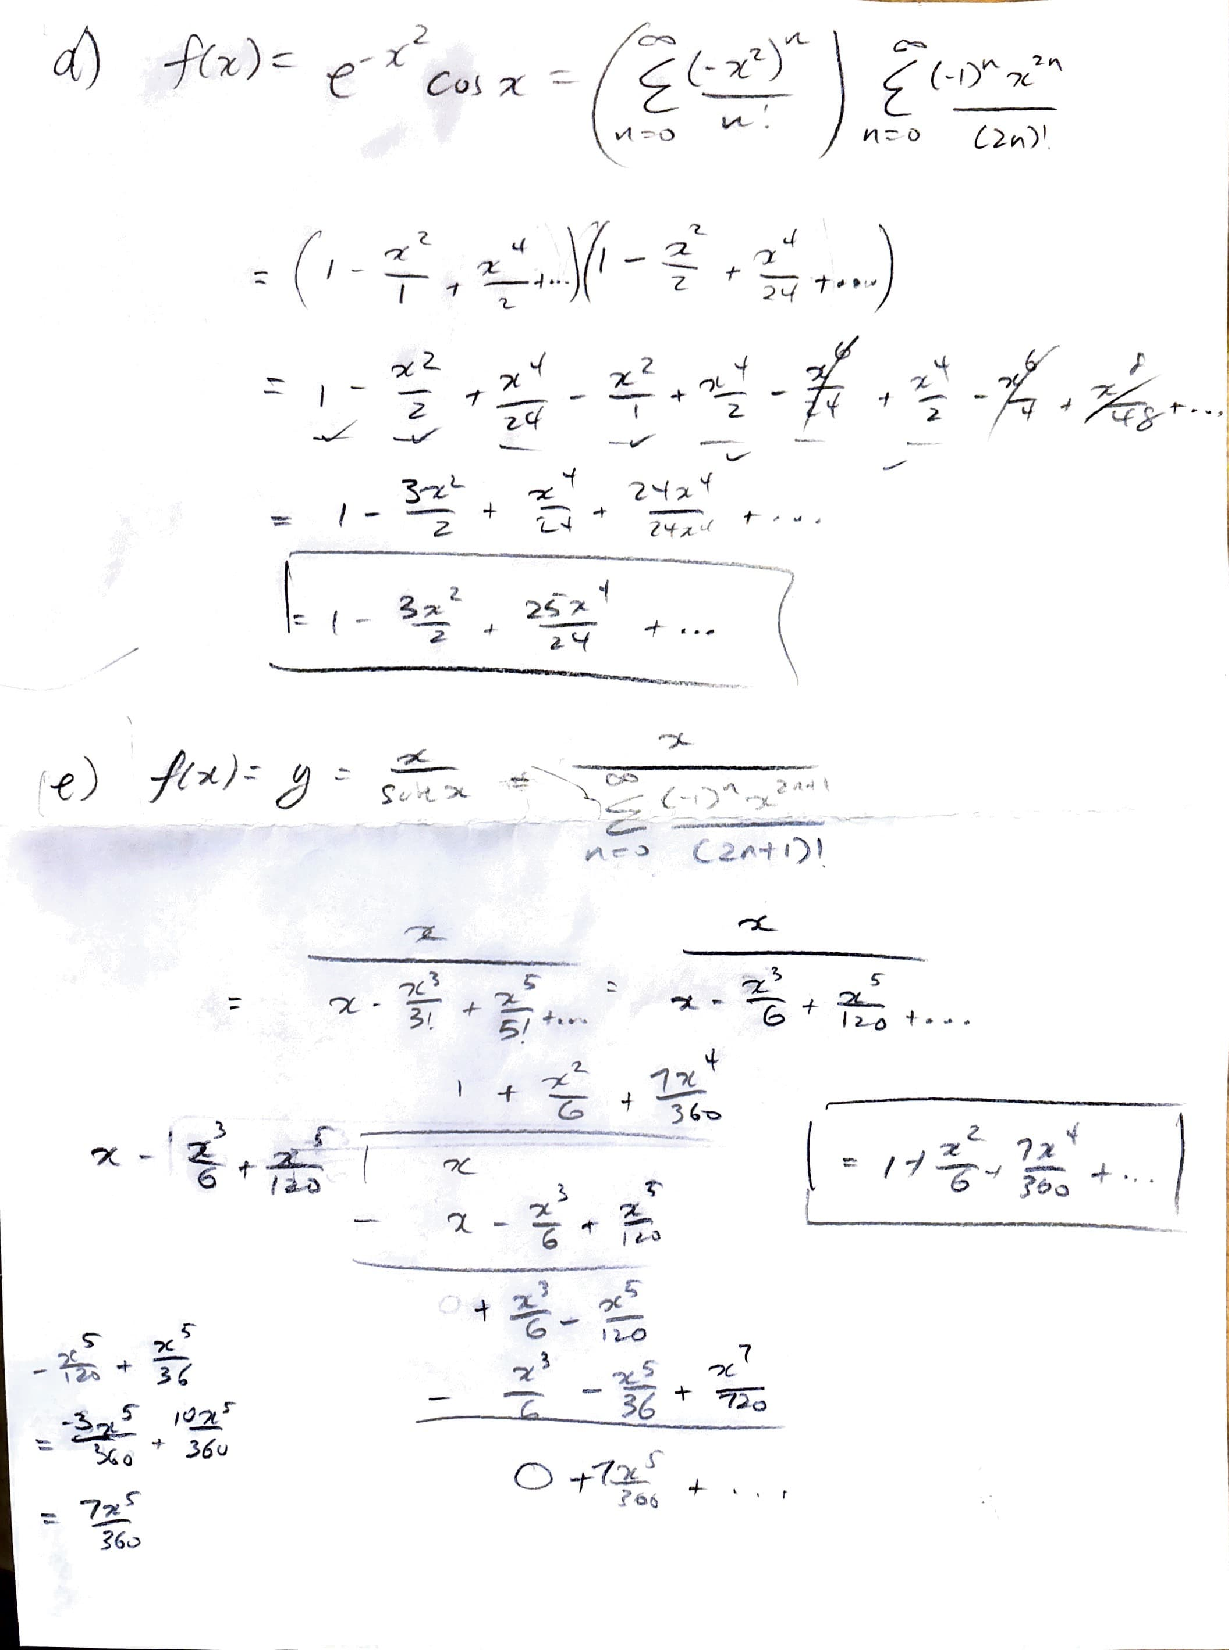
\includegraphics[scale=0.75, page=1]{q6.pdf}
	\includegraphics[scale=0.58, page=2]{q6.pdf}
\end{center}

\end{document}
